\subsection{\labeltext[UC02 - Administração]{UC2.1 - Gerir Conta}{uc:21}}
A imagem identificada como figura~\ref{fig:chap212} apresenta o diagrama de caso de uso \ref{uc:21} e tem como objetivo apresentar as interações entre os atores e o sistema.

\vspace*{5mm}

\begin{figure}[H]
	\centering
	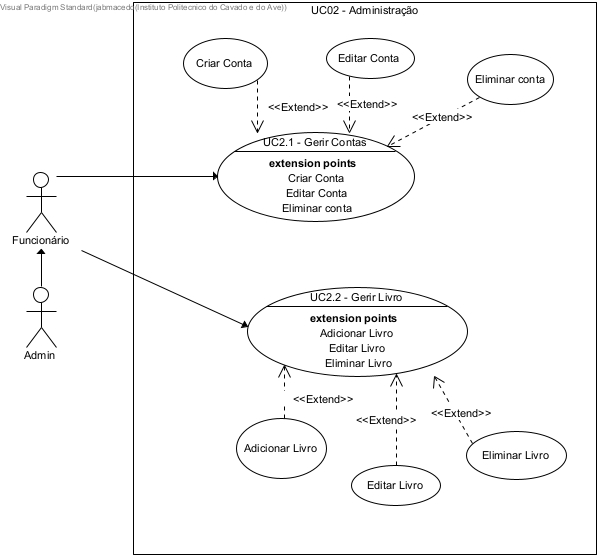
\includegraphics[width=1\linewidth]{./img/Diagramas\_UC/UC02.jpg}  % largura percentual 
	\caption{\ref{uc:21}}
	\label{fig:chap212}
\end{figure}

\newpage

\noindent \textbf{Descrição} \\
\textbf{ID:} UC2.1 \\  
\textbf{Nível de importância:} Alta \\
\textbf{Nome:} Gerir Conta \\
\textbf{Ator principal:} Utilizador \\
\textbf{Atores secundários:} --------- \\
\textbf{Breve descrição:} O utilizador poderá editar e eliminar conta. \\ 
\textbf{Ativador:} Intenção do utilizador querer editar a sua conta.  \\
\textbf{Pré-condições:} Ter conta criada. \\
\textbf{Fluxo normal dos eventos:} \\
1. Abrir sistema.  \\
2. Autenticar-se no sistema. \\
3. Selecionar "Conta" \\
\textbf{Sub-fluxos:} \\ 
\indent A - Editar conta\\
	\indent\indent A.1 - Este sub-fluxo inicia quando o utilizador deseja editar conta.\\
	\indent\indent A.2 - O utilizador insere os dados nos campos onde quer alterar.\\	
	\indent\indent A.3 - O utilizador carrega no botão "Registar".\\	
	\indent\indent A.4 - O sistema guarda os dados na base de dados e encaminha para o menu principal.\\	
	\indent B - Apagar conta \\ 
	\indent\indent B.1 - Este sub-fluxo inicia quando o utilizador deseja apagar a sua conta do sistema.\\
	\indent\indent B.2 - O sistema uma mensagem de confirmação da ação.\\
	\indent\indent B.3 - O utilizador confirma a operação.\\
	\indent\indent B.4 - O sistema guarda os dados na base de dados e encaminha o utilizador para a página inicial do sistema.\\
\textbf{Fluxos alternativos/excecionais:}  \\
	\indent A qualquer momento antes de submeter, o utilizador pode selecionar cancelar. A ação não é gravado e o caso de uso termina.\\
	\indent A - Editar conta\\
	\indent\indent A.5 - Se alguma informação estiver incorreta, o sistema pede ao utilizador para corrigir a informação.\\

\newpage

\subsection{UC2.2 - Gerir livro}
\vspace*{5mm}

\noindent \textbf{Descrição} \\
\textbf{ID:} UC2.2 \\  
\textbf{Nível de importância:} Alta \\
\textbf{Nome:} Gerir livro \\
\textbf{Ator principal:} Funcionário e/ou Administrador \\
\textbf{Atores secundários:} --------- \\
\textbf{Breve descrição:} O Funcionário e/ou Administrador deverão conseguir inserir, ediar e remover livros do sistema \\ 
\textbf{Ativador:} Necessidade do Funcionário e/ou Administrador dar entrada, editar dados e/ou apagar um livro. \\
\textbf{Pré-condições:} Ter nível de permissão de Funcionário e/ou Administrador. \\
\textbf{Fluxo normal dos eventos:} \\
	\indent Caso de uso inicia quando o Funcionário e/ou Administrador deseja gerir livros. \\
	\indent De acordo com o tipo de operação que deseja efetuar é encaminhado para os seguintes sub-fluxo:\\
	\indent\indent A - Se o utilizador deseja criar/inserir um livro, o sub-fluxo "Inserir" é executado.\\
	\indent\indent B - Se o utilizador deseja editar um livro, o sub-fluxo "Editar" é executado.\\
	\indent\indent C - Se o utilizador deseja remover um livro, o sub-fluxo "Remover" é executado.\\
\textbf{Sub-fluxos:} \\
	\indent A - Inserir livro\\
	\indent\indent A.1 - Este sub-fluxo inicia quando o utilizador deseja inserir um livro.\\
	\indent\indent A.2 - O utilizador insere os dados nos campos necessários.\\	
	\indent\indent A.3 - O utilizador carrega no botão "Registar".\\	
	\indent\indent A.4 - O sistema guarda os dados na base de dados e encaminha para o menu gerir livros.\\	
	\indent B - Editar livro \\ 
	\indent\indent B.1 - Este sub-fluxo inicia quando o utilizador deseja alterar informação de um livro.\\
	\indent\indent B.2 - É apresentado ao utilizador a lista de livros.\\
	\indent\indent B.3 - O utilizador edita os dados dos campos a editar.\\
	\indent\indent B.4 - O utilizador carrega no botão Atualizar.\\
	\indent\indent B.5 - O sistema guarda os dados na base de dados e encaminha para o menu gerir livros.\\
	\indent C -Remover livro  \\
	\indent\indent C.1 - Este sub-fluxo inicia quando o utilizador deseja remover um livro.\\
	\indent\indent C.2 - O sistema apresenta a lista de livros.\\
	\indent\indent C.3 - O utilizador seleciona livro que deseja remover.\\
	\indent\indent C.4 - O sistema responde com uma mensagem "livro removido com sucesso." e encaminha para o menu gerir livros.\\
\textbf{Fluxos alternativos/excecionais:}  \\
	\indent A qualquer momento antes de submeter, o utilizador pode selecionar cancelar. A ação não é gravado e o caso de uso termina.\\
	\indent A - Inserir livro\\
	\indent\indent A.5 - Se alguma informação estiver incorreta, o sistema pede ao utilizador para corrigir a informação.\\
	\indent B - Editar livro\\
	\indent\indent B.6 - Se alguma informação estiver incorreta, o sistema pede ao utilizador para corrigir a informação.\\